\documentclass[12pt]{article}
\usepackage{caption}
\usepackage{float}
\usepackage{graphicx}
\usepackage{fancyhdr}
\pagestyle{fancy}
\pagenumbering{Roman}
\renewcommand{\headrulewidth}{1pt}
\renewcommand{\footrulewidth}{1pt}
\setlength{\headheight}{25pt}
\rhead{\textbf{Lightning Coalition Robotics}}
\cfoot{}
\rfoot{\thepage}
\begin{document}

% Add date (e.g. September 14, 2018) and then your name/all authors.
October 13 - Chris Lonergan

\section{Our Plan:}
\begin{itemize}
% After \item, add what you want for the bullet point. (\item adds a new bullet point when you run out.)
	\item Drive Chain
	\item Arm
	\item Design mechanism to pick minerals off the ground
\end{itemize}

We wanted to do the tank treads, and test them as well. We also wanted to design a mechanism for our arm that picks the robot up and we wanted to design a mechanism to pick "minerals" off the ground.

\section{What We Got Done:}

Today, we assembled the tank treads and tested them. We also designed a worm gear and motor CAD file for the robot assembly.

%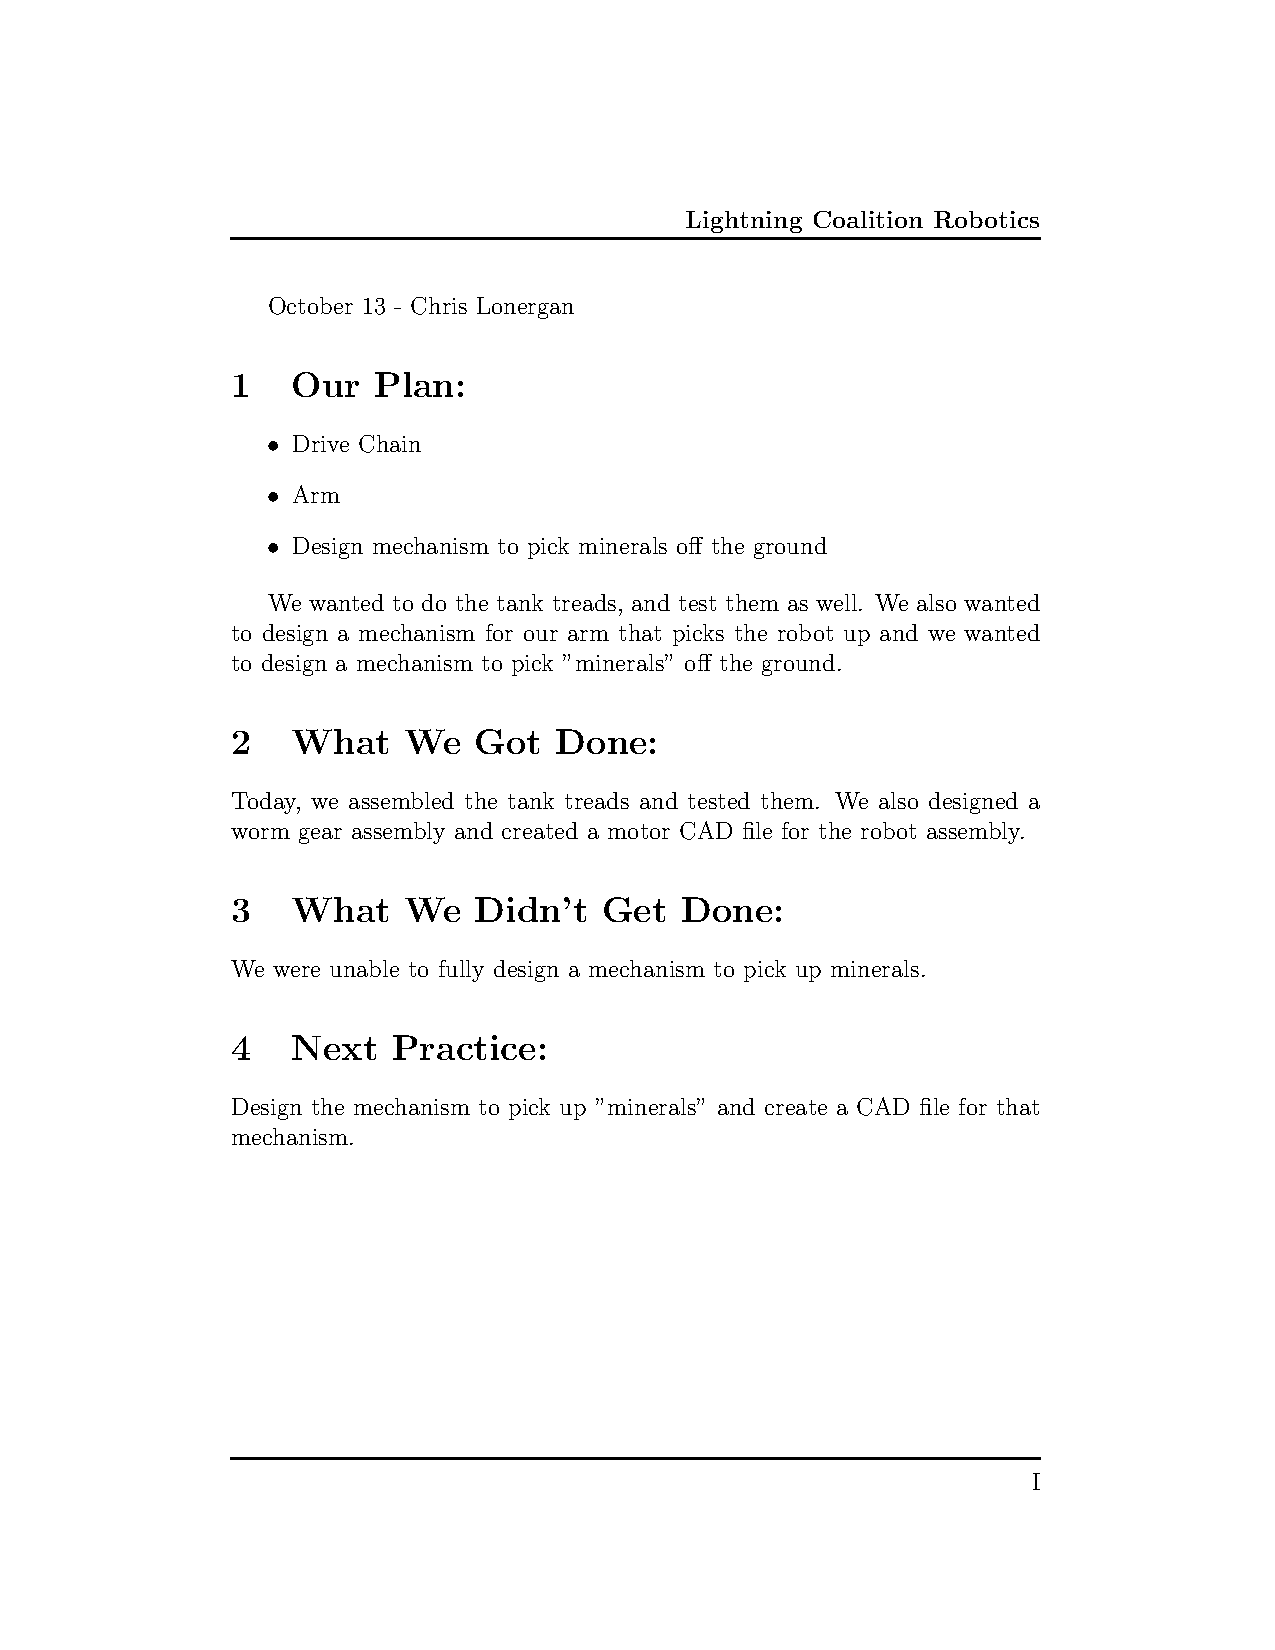
\includegraphics[scale=1]{october13.png}%image

\section{What We Didn't Get Done:}

We were unable to fully design a mechanism to pick up minerals.

\section{Next Practice:}
Design the mechanism to pick up "minerals" and create a CAD file.


\end{document}
